
\chapter{STF多级展开}

\section{符号约定}

引入指标分配符号 \((i_1, \dots, i_n)\)，对于 \(q_i\) 个 \(p_i\) 阶对称张量 \(T^{[i](p_i)}\)(\(i=1,\dots,m,\,n=\sum_{i=1}^m q_i p_i \))
\begin{align*}
	T^{[1](p_1)}_{(i_1 \dots i_{p_1}} \dots T^{[m](p_m)}_{i_{n-p_m+1} \dots i_n)}
\end{align*}
指将 \(i_1\) 至 \(i_n\) 按照完全不重复的方式分配给这 \(\sum_{i=1}^m q_i\) 个张量，再对所分配的 \(n!/\prod_{i=1}^m (q_i! (p_i!)^{q_i})\) 个结果求和.

比如，\(\delta_{(i_1i_2}f_{i_3)}=\delta_{i_1i_2}f_{i_3}+\delta_{i_2i_3}f_{i_1}+\delta_{i_3i_1}f_{i_2}\)，给出\(n=3,\,q_1=q_2=1,\,p_1=2,\,p_2=1\)，因此有3项.比如，\(\nabla_{(i_1}\nabla_{i_2}\nabla_{i_3)}=\nabla_{i_1}\nabla_{i_2}\nabla_{i_3}\)，给出\(n=3,\,q_1=3,\,p_1=1\)，因此有1项.比如，对于对称二阶张量\(T\)，\(T\)不是\(\delta\)记号，\(\delta_{(i_1 i_2}T_{i_3 i_4)}=\delta_{i_1 i_2}T_{i_3 i_4}+\delta_{i_1 i_3}T_{i_2 i_4}+\delta_{i_1 i_4}T_{i_2 i_3}+\delta_{i_2 i_3}T_{i_1 i_4}+\delta_{i_2 i_4}T_{i_1 i_3}+\delta_{i_3 i_4}T_{i_1 i_2}\)，给出\(n=4,\,q_1=q_2=1,\,p_1=2,\,p_2=2\)，因此有6项；而如果\(T\)是\(\delta\)记号，\(\delta_{(i_1 i_2}\delta_{i_3 i_4)}=\delta_{i_1 i_2}\delta_{i_3 i_4}+\delta_{i_1 i_3}\delta_{i_2 i_4}+\delta_{i_1 i_4}\delta_{i_2 i_3}\)，给出\(n=4,\,q_1=2,\,p_1=2\)，因此有3项.还比如，记 \(T^{(n-2m)}\) 是一个 \(n-2m\) 阶的对称张量，则 \(\delta_{(i_1 i_2} \dots \delta_{i_{2m-3} i_{2m-2}} T^{(n-2m)}_{i_{2m-1} \dots i_{n-2})}\) 对应 \(q_1 = m-1\)，\(p_1 = 2\)，\(q_2 = 1\)，\(p_2 = n-2m\)，式中共有 \(n!/(2^{m-1} (m-1)! (n-2m)!)\) 项.

引入对称化操作算符 \(\mathcal{S}\)，对于任意 \(n\) 阶张量 \(T^{(n)}\)，设其有 \(m\) 类指标、每类指标有 \(p_i\)(\(\,i=1,\dots,m,\,\sum_{i=1}^mp_i=n,\,p_i\geq 1\))个是对称的，则：
\begin{align*}
	\mathcal{S} T^{(n)} = T_{(i_1 \dots i_n)}\frac{1}{n!} \prod_{i=1}^m p_i!.
\end{align*}
严格地说，这里运用指标分配符号时并不存在多个对称张量，但是存在某一张量的多类对称位置（矢量也是对称张量），仍适用于如上讨论.另外易知，\(\mathcal{S} T^{(n)}\) 是 \(n\) 阶对称张量.
\begin{note}
	对称化算符也可以写作更直观的全置换形式
	\begin{align*}
		\mathcal{S} T^{(n)} = \frac{1}{n!}\sum_{\rm a.p.} T_{i_1 \dots i_n}
	\end{align*}
	其中“a.p.=all permutations”指\(i_1\)至\(i_n\)的全部\(n!\)种置换。
\end{note}

由于以下讨论的张量都具有较高的对称性，若每一次计算都要相加\(n!\)个置换值则过于麻烦且不直观，因此引入了\(T_{(i_1 \dots i_n)}\)记号。特别注意，在有些书中，\(T_{(i_1 \dots i_n)}\)被定义为本文的\(\mathcal{S} T^{(n)}\)，阅读时应加以区分。

引入对称无迹操作算符 \(\mathcal{STF}\)，对于任意 \(n\) 阶张量 \(T^{(n)}\)：
\begin{align*}
	\mathcal{STF} T^{(n)} = \mathcal{S} T^{(n)} - \delta_{(i_1 i_2} \Lambda[\mathcal{S} T^{(n)}]_{i_3 \dots i_n)},
\end{align*}
这里的 \(\Lambda\) 算符可将对称张量的阶数降下2，具体而言：
\begin{align*}
	\Lambda[\mathcal{S} T^{(n)}] = \sum_{m=1}^{\lfloor n/2 \rfloor} \frac{(-1)^{m-1} (2n - 1 - 2m)!!}{m (2n - 1)!!} \delta_{(i_1 i_2} \dots \delta_{i_{2m-3} i_{2m-2}} \mathcal{S} T^{(n.m)}_{i_{2m-1} \dots i_{n-2})}.
\end{align*}
其中 \(\mathcal{S}T^{(n.m)}\) 指将 \(n\) 阶对称张量 \(\mathcal{S}T^{(n)}\) 中的 \(m\) 对指标缩并.不难验证，\(\mathcal{STF}T^{(n)}\) 是 \(n\) 阶对称无迹张量.由于 \(\mathcal{STF}\) 作用于矢量或标量仍得其本身，上式还可写作：
\begin{align*}
	\mathcal{S}T^{(n)} = \sum_{m=1}^{\lfloor n/2 \rfloor} \delta_{(i_1 i_2} \dots \delta_{i_{2m-1} i_{2m}} \left( \mathcal{STF}\Lambda^{\otimes m}[\mathcal{S}T^{(n)}] \right)_{i_{2m+1} \dots i_n)},
\end{align*}
\(\lfloor \cdot \rfloor\) 是向下取整符号.

\section{原始多极矩的导出}
先介绍赫兹矢量法，该法可通过电磁极化强度求解电磁场.

当空间中存在局域电极化强度 \(\vb{P}\) 及磁化强度 \(\vb{M}\)，且无自由电荷、自由电流时（在辐射问题中，自由电荷、自由电流不会贡献远场辐射功率，因此也不妨忽略）：
\begin{align*}
	\vb{D} = \varepsilon_0 \vb{E} + \vb{P}, \quad \vb{B} = \mu_0 \left( \vb{H} + \vb{M} \right), \quad \nabla \cdot \vb{D} = 0, \quad \nabla \times \vb{H} = \frac{\partial \vb{D}}{\partial t}.
\end{align*}

引入电势 \(\Phi\)、磁矢势 \(\vb{A}\) 及相应的洛伦兹规范，使得电磁场满足
\begin{align*}
	\vb{E} = -\nabla \Phi - \frac{\partial \vb{A}}{\partial t}, \quad \vb{B} = \nabla \times \vb{A}, \quad \nabla \cdot \vb{A} + \frac{1}{c^2}\frac{\partial \Phi}{\partial t} = 0.
\end{align*}

代入得
\begin{align*}
	\left( \nabla^2 - \frac{\partial^2}{c^2 \partial t^2} \right) \Phi = \frac{1}{\varepsilon_0} \nabla \cdot \vb{P}, \quad \left( \nabla^2 - \frac{\partial^2}{c^2 \partial t^2} \right) \vb{A} = -\mu_0 \left( \frac{\partial \vb{P}}{\partial t} + \nabla \times \vb{M} \right).
\end{align*}

引入赫兹矢量 \(\vb{\Pi}_e, \vb{\Pi}_m\)，使得
\begin{align*}
	\vb{A} = \mu_0 \left( \frac{\partial \vb{\Pi}_e}{\partial t} + \nabla \times \vb{\Pi}_m \right), \quad \Phi = -\frac{1}{\varepsilon_0} \nabla \cdot \vb{\Pi}_e.
\end{align*}

代入得
\begin{align*}
	&\nabla \cdot \left( \nabla^2 \vb{\Pi}_e - \frac{\partial^2 \vb{\Pi}_e}{c^2 \partial t^2} + \vb{P} \right) = 0, \\
	&\frac{\partial}{\partial t} \left( \nabla^2 \vb{\Pi}_e - \frac{\partial^2 \vb{\Pi}_e}{c^2 \partial t^2} + \vb{P} \right) + \nabla \times \left( \nabla^2 \vb{\Pi}_m - \frac{\partial^2 \vb{\Pi}_m}{c^2 \partial t^2} + \vb{M} \right) = 0.
\end{align*}

该式的解可写作（\(\vb{V}, \xi\) 为任意函数）
\begin{align*}
	\nabla^2 \vb{\Pi}_e - \frac{\partial^2 \vb{\Pi}_e}{c^2 \partial t^2} &= -\vb{P} + \nabla \times \vb{V}, \\
	\nabla^2 \vb{\Pi}_m - \frac{\partial^2 \vb{\Pi}_m}{c^2 \partial t^2} &= -\vb{M} - \frac{\partial \vb{V}}{\partial t} + \nabla \left( \frac{\partial \xi}{\partial t} \right).
\end{align*}

注意到，引入赫兹矢量后，电势、磁矢势仍满足洛伦兹规范，且规范变换
\begin{align*}
	\vb{A} \to \vb{A} + \nabla \Lambda, \quad \Phi \to \Phi - \frac{\partial \Lambda}{\partial t}, \quad \left( \nabla^2 - \frac{\partial^2}{c^2 \partial t^2} \right) \Lambda = 0.
\end{align*}
可以写作
\begin{align*}
	\vb{\Pi}_e \to \vb{\Pi}_e + \nabla \times \vb{G} - \nabla g_e, \quad \vb{\Pi}_m \to \vb{\Pi}_m - \frac{\partial \vb{G}}{\partial t} - \nabla g_m.
\end{align*}
其中 \(g_m, \vb{G}\) 可任取，\(\left( \nabla^2 - \partial^2/c^2 \partial t^2 \right) g_e = 0\).不妨取
\begin{align*}
	\left( \nabla^2 - \frac{\partial^2}{c^2 \partial t^2} \right) \vb{G} = -(\vb{V} + \nabla \xi), \quad g_m = 0.
\end{align*}

则规范变换后的赫兹矢量满足
\begin{align*}
	\nabla^2 \vb{\Pi}_e - \frac{\partial^2 \vb{\Pi}_e}{c^2 \partial t^2} = -\vb{P}, \quad \nabla^2 \vb{\Pi}_m - \frac{\partial^2 \vb{\Pi}_m}{c^2 \partial t^2} = -\vb{M}.
\end{align*}

若已知局域电极化强度、磁化强度分布，则可根据上式求出赫兹矢量，再根据下式求出电磁场：
\begin{align*}
	\vb{A} &= \mu_0 \left( \frac{\partial \vb{\Pi}_e}{\partial t} + \nabla \times \vb{\Pi}_m \right), \quad \Phi = -\frac{1}{\varepsilon_0} \nabla \cdot \vb{\Pi}_e. \\
	\vb{E} &= -\nabla \Phi - \frac{\partial \vb{A}}{\partial t} = \frac{1}{\varepsilon_0} \nabla \left( \nabla \cdot \vb{\Pi}_e \right) - \mu_0 \left( \frac{\partial^2 \vb{\Pi}_e}{\partial t^2} + \nabla \times \left( \frac{\partial \vb{\Pi}_m}{\partial t} \right) \right), \\
	\vb{B} &= \nabla \times \vb{A} = \mu_0 \left( \nabla \times \left( \frac{\partial \vb{\Pi}_e}{\partial t} \right) + \nabla \times \left( \nabla \times \vb{\Pi}_m \right) \right).
\end{align*}

下具体求出 \(\vb{P}, \vb{M}\) 和局域电荷分布的关系.假设电荷在 \(\vb{r}_s\) 点附近分布，该点以速度 \(\vb{v}_s = d\vb{r}_s/dt\) 运动，各电荷相对 \(\vb{r}_s\) 的位矢为 \(\vb{r}'\)，相对其的运动速度为 \(\vb{v}' = \dd \vb{r}'/dt\).
宏观上，所有电荷都近似集中在 \(\vb{r}_s\)，空间电流也由 \(\vb{r}_s\) 的变化引起；微观上，则要考虑电荷关于 \(\vb{r}_s\) 的分布，即：
\begin{align*}
	\nabla \cdot \vb{E} &= \frac{1}{\varepsilon_0} \int \rho\!\left( \vb{r}' + \vb{r}_s, t \right) \delta\!\left( \vb{r} - \vb{r}' - \vb{r}_s \right) \dd \vb{r}', \\
	\nabla \cdot \vb{D} &= \int \rho\!\left( \vb{r}' + \vb{r}_s, t \right) \delta\!\left( \vb{r} - \vb{r}_s \right) \dd \vb{r}', \\
	\nabla \times \vb{B} &= \frac{1}{c^2} \frac{\partial \vb{E}}{\partial t} + \mu_0 \int \rho\!\left( \vb{r}' + \vb{r}_s, t \right) \left( \vb{v}_s + \vb{v}' \right) \delta\!\left( \vb{r} - \vb{r}' - \vb{r}_s \right) \dd \vb{r}', \\
	\nabla \times \vb{H} &= \frac{\partial \vb{D}}{\partial t} + \int \rho\!\left( \vb{r}' + \vb{r}_s, t \right) \vb{v}_s \delta\!\left( \vb{r} - \vb{r}_s \right) \dd \vb{r}'.
\end{align*}
其中 \(\dd \vb{r}'\) 是源的体积元.

记 \(\vb{r}\) 的 \(n\) 次并矢为 \(\vb{r}^{\otimes n}\)，用单个点乘表示 \(\vb{r}^{\otimes n}\) 的 \(n\) 个指标与其后张量的前 \(n\) 个张量的缩并（由于以下讨论中“其后张量”需要缩并的指标都是对称的，因此这样表示不会引起歧义），\(\nabla^{\otimes n}\) 同理.

根据泰勒展开：
\begin{align*}
	\delta\!\left( \vb{r} - \vb{r}' - \vb{r}_s \right)
	= \sum_{n=0}^{\infty} \frac{(-1)^n}{n!}\,
	\vb{r}'^{\otimes n} \cdot \nabla^{\otimes n} \delta\!\left( \vb{r} - \vb{r}_s \right).
\end{align*}

并记 \(\vb{P} = \vb{D} - \varepsilon_0 \vb{E}\)，\(\vb{M} = -\vb{H} + \vb{B}/\mu_0\)，得：
\begin{align*}
	\nabla \cdot \vb{P}
	&= \nabla \cdot \left( \vb{D} - \varepsilon_0 \vb{E} \right)
	= \sum_{n=1}^{\infty} \frac{(-1)^{n-1}}{n!}
	\int \rho\!\left( \vb{r}' + \vb{r}_s, t \right)
	\vb{r}'^{\otimes n} \cdot \nabla^{\otimes n}
	\delta\!\left( \vb{r} - \vb{r}_s \right) \dd \vb{r}' \\
	&\to \vb{P}
	= \sum_{n=1}^{\infty} \frac{(-1)^{n-1}}{n!}
	\int \rho\!\left( \vb{r}' + \vb{r}_s, t \right)
	\vb{r}'^{\otimes n} \cdot \nabla^{\otimes (n-1)}
	\delta\!\left( \vb{r} - \vb{r}_s \right) \dd \vb{r}', \\
	\nabla \times \vb{M}
	&= \nabla \times \left( -\vb{H} + \frac{\vb{B}}{\mu_0} \right)
	= -\frac{\partial \vb{P}}{\partial t} + \vb{v}_s \nabla \cdot \vb{P}
	+ \sum_{n=1}^{\infty} \frac{(-1)^n}{n!}
	\int \rho\!\left( \vb{r}' + \vb{r}_s, t \right)
	\vb{v}' \vb{r}'^{\otimes n} \cdot \nabla^{\otimes n}
	\delta\!\left( \vb{r} - \vb{r}_s \right) \dd \vb{r}' \\
	&\to \vb{M}
	= \sum_{n=1}^{\infty} \frac{(-1)^{n-1}}{n!} \cdot \frac{n}{n+1}
	\int \rho\!\left( \vb{r}' + \vb{r}_s, t \right)
	\left( \vb{r}' \times \vb{v}' \right)
	\vb{r}'^{\otimes (n-1)} \cdot \nabla^{\otimes (n-1)}
	\delta\!\left( \vb{r} - \vb{r}_s \right) \dd \vb{r}'.
\end{align*}

记原始电 \(2^n\) 极矩、原始磁 \(2^n\) 极矩为：
\begin{align*}
	P^{(n)}(t) &= \int \rho\left( \vb{r}' + \vb{r}_s, t \right) \vb{r}'^{\otimes n} \dd \vb{r}', \quad
	M^{(n)}(t) = \frac{n}{n+1} \int \vb{r}'^{\otimes (n-1)} \left( \vb{r}' \times \vb{J}\left( \vb{r}' + \vb{r}_s, t \right) \right) \dd \vb{r}'.
\end{align*}
其中用到 \(\vb{J}\left( \vb{r}' + \vb{r}_s, t \right) = \rho\left( \vb{r}' + \vb{r}_s, t \right) \vb{v}'\).进而：
\begin{align*}
	\vb{P} &= \sum_{n=1}^{\infty} \frac{(-1)^{n-1}}{n!} \nabla^{\otimes (n-1)} \cdot \left( P^{(n)}(t) \delta\left( \vb{r} - \vb{r}_s \right) \right), \quad
	\vb{M} = \sum_{n=1}^{\infty} \frac{(-1)^{n-1}}{n!} \nabla^{\otimes (n-1)} \cdot \left( M^{(n)}(t) \delta\left( \vb{r} - \vb{r}_s \right) \right).
\end{align*}

根据赫兹矢量法：
\begin{align*}
	\nabla^2 \vb{\Pi}_e - \frac{\partial^2 \vb{\Pi}_e}{c^2 \partial t^2} = -\vb{P}, \quad \nabla^2 \vb{\Pi}_m - \frac{\partial^2 \vb{\Pi}_m}{c^2 \partial t^2} = -\vb{M}.
\end{align*}

在三维无界空间中，上式的解为：
\begin{align*}
	\vb{\Pi}_e(\vb{r}, t) &= \frac{1}{4\pi} \int \frac{\vb{P}\left( \vb{r}', t - \dfrac{|\vb{r} - \vb{r}'|}{c} \right)}{|\vb{r} - \vb{r}'|} \dd \vb{r}' = \frac{1}{4\pi} \sum_{n=1}^{\infty} \frac{(-1)^{n-1}}{n!} \nabla^{\otimes (n-1)} \cdot \frac{P^{(n)}(t-r/c)}{r}, \\
	\vb{\Pi}_m(\vb{r}, t) &= \frac{1}{4\pi} \int \frac{\vb{M}\left( \vb{r}', t - \dfrac{|\vb{r} - \vb{r}'|}{c} \right)}{|\vb{r} - \vb{r}'|} \dd \vb{r}' = \frac{1}{4\pi} \sum_{n=1}^{\infty} \frac{(-1)^{n-1}}{n!} \nabla^{\otimes (n-1)} \cdot \frac{M^{(n)}(t-r/c)}{r}.
\end{align*}

对应空间中的电磁势为（注意以下所有源相关物理量均在\(t-r/c\)时刻取值）：
\begin{align*}
	\vb{A} &= \mu_0 \left( \frac{\partial \vb{\Pi}_e}{\partial t} + \nabla \times \vb{\Pi}_m \right) = \frac{\mu_0}{4\pi} \sum_{n=1}^{\infty} \frac{(-1)^{n-1}}{n!} \left( \nabla^{\otimes (n-1)} \cdot \frac{\partial P^{(n)}}{r \partial t} + \nabla \times \left( \nabla^{\otimes (n-1)} \cdot \frac{M^{(n)}}{r} \right) \right), \\
	\Phi &= -\frac{1}{\varepsilon_0} \nabla \cdot \vb{\Pi}_e = -\frac{1}{4\pi\varepsilon_0} \sum_{n=1}^{\infty} \frac{(-1)^{n-1}}{n!} \nabla^{\otimes n} \cdot \frac{P^{(n)}}{r}.
\end{align*}

该形式较为简便且直观，但注意到辐射场通常只包括多极矩的对称无迹（STF/symmetric trace free，指任意两个指标交换对称、缩并得零，矢量一定是STF）部分，因此还可以用一套数学办法将上式STF化.

\section{对称无迹化的具体步骤}
根据上面关于电或磁极化的讨论，记：
\begin{align*}
	P^{(n)} &= \int \rho \vb{r}'^{\otimes n} \dd \vb{r}', \quad
	M^{(n)} = \frac{n}{n+1} \int \vb{r}'^{\otimes (n-1)} \left( \vb{r}' \times \vb{J} \right) \dd \vb{r}'.
\end{align*}
另外定义：
\begin{align*}
	M^{(n.m)} &= \frac{n}{n+1} \int (r')^{2m} \vb{r}'^{\otimes (n-2m-1)} \left( \vb{r}' \times \vb{J} \right) \dd \vb{r}', \\
	N^{(n)} &= \frac{n+1}{n+2} \int \vb{r}'^{\otimes (n-1)} \left( \vb{r}' \times \left( \vb{r}' \times \vb{J} \right) \right) \dd \vb{r}', \quad
	N^{(n.m)} = \frac{n+1}{n+2} \int (r')^{2m} \vb{r}'^{\otimes (n-2m-1)} \left( \vb{r}' \times \left( \vb{r}' \times \vb{J} \right) \right) \dd \vb{r}'.
\end{align*}

不难看到：
\begin{align*}
	\mathcal{S}M^{(n)} &= M^{(n)} - \frac{1}{n} \sum_{p=1}^{n-1} \epsilon_{i_p i_n q} N^{(n-1)}_{i_1 \dots i_{p-1} i_{p+1} \dots i_{n-1} q}, \\
	\mathcal{S}N^{(n-1)} &= N^{(n-1)} + \frac{1}{n-1} \sum_{p=1}^{n-2} \epsilon_{i_p i_n q} M^{(n.1)}_{i_1 \dots i_{p-1} i_{p+1} \dots i_{n-2} q}.
\end{align*}

进而（下式 \(\Delta = \nabla^2\)）：
\small
\begin{align*}
	\nabla^{\otimes (n-1)} \cdot \left( \frac{P^{(n)}}{r} \right) &= \nabla^{\otimes (n-1)} \cdot \left( \frac{\mathcal{STF}P^{(n)}}{r} \right) + (n-1) \nabla \left( \nabla^{\otimes (n-2)} \cdot \left( \frac{\Lambda[P^{(n)}]}{r} \right) \right) + \frac{(n-2)(n-1)}{2} \Delta \nabla^{\otimes (n-3)} \cdot \left( \frac{\Lambda[P^{(n)}]}{r} \right) \\
	&= \sum_{m=0}^{\lfloor \frac{n-1}{2} \rfloor} \frac{(n-1)!}{2^m (n-2m-1)!} \Delta^m \nabla^{\otimes (n-2m-1)} \cdot \frac{\mathcal{STF}\Lambda^{\otimes m}[P^{(n)}]}{r} + \nabla \left( f_e \frac{1}{r} \right),
\end{align*}

\begin{align*}
	\nabla^{\otimes (n-1)}& \cdot \left( \frac{M^{(n)}}{r} \right) = \nabla^{\otimes (n-1)} \cdot \left( \frac{\mathcal{S}M^{(n)}}{r} \right) - \frac{n-1}{n} \nabla \times \left( \nabla^{\otimes (n-2)} \cdot \left( \frac{\mathcal{S}N^{(n-1)}}{r} \right) \right) \\&\hspace{2cm}+ \frac{n-2}{n} \Delta \nabla^{\otimes (n-3)} \cdot \left( \frac{\mathcal{S}M^{(n.1)}}{r} \right) - \frac{n-2}{n} \nabla \left( \nabla^{\otimes (n-2)} \cdot \left( \frac{\mathcal{S}M^{(n.1)}}{r} \right) \right)\\
	&= \sum_{m=0}^{\lfloor \frac{n-1}{2} \rfloor} \frac{n-2m}{n} \Delta^m \nabla^{\otimes (n-2m-1)} \cdot \frac{\mathcal{S}M^{(n.m)}}{r} - \nabla \times \sum_{m=0}^{\lfloor \frac{n-2}{2} \rfloor} \frac{n-2m-1}{n} \Delta^m \nabla^{\otimes (n-2m-2)} \cdot \frac{\mathcal{S}N^{(n-1.m)}}{r} + \nabla \left( \tilde{f}_m \cdot \frac{1}{r} \right) \\
	&= \sum_{m=0}^{\lfloor \frac{n-1}{2} \rfloor} \sum_{k=0}^{\lfloor \frac{n-2m-1}{2} \rfloor} \frac{(n-2m)!}{2^k n (n-2m-1-2k)!} \Delta^{m+k} \nabla^{\otimes (n-2m-2k-1)} \cdot \frac{\mathcal{STF}\Lambda^{\otimes k}[\mathcal{S}M^{(n.m)}]}{r} \\
	&\quad - \nabla \times \sum_{m=0}^{\lfloor \frac{n-2}{2} \rfloor} \sum_{k=0}^{\lfloor \frac{n-2m-2}{2} \rfloor} \frac{(n-2m-1)!}{2^k n (n-2m-2-2k)!} \Delta^{m+k} \nabla^{\otimes (n-2m-2k-2)} \cdot \frac{\mathcal{STF}\Lambda^{\otimes k}[\mathcal{S}N^{(n-1.m)}]}{r} + \nabla \left( f_m  \frac{1}{r} \right) \\
	&= \sum_{m=0}^{\lfloor \frac{n-1}{2} \rfloor} \sum_{k=0}^m \frac{(n-2m+2k)!}{2^k n (n-2m-1)!} \Delta^m \nabla^{\otimes (n-2m-1)} \cdot \frac{\mathcal{STF}\Lambda^{\otimes k}[\mathcal{S}M^{(n.m-k)}]}{r} \\
	&\quad - \nabla \times \sum_{m=0}^{\lfloor \frac{n-2}{2} \rfloor} \sum_{k=0}^m \frac{(n-2m+2k-1)!}{2^k n (n-2m-2)!} \Delta^m \nabla^{\otimes (n-2m-2)} \cdot \frac{\mathcal{STF}\Lambda^{\otimes k}[\mathcal{S}N^{(n-1.m-k)}]}{r} + \nabla \left( f_m  \frac{1}{r} \right).
\end{align*}
\normalsize
其中 \(f_e, \tilde{f}_m, f_m\) 是 \(\nabla\) 的函数，而对该类型函数，\(\left( \Delta - \partial^2/c^2 \partial t^2 \right) \left( f_e/r \right) = 0\)，因此 \(f_e, f_m\) 项可通过赫兹矢量的规范变换\(\vb{\Pi}_e \to \vb{\Pi}_e + \nabla \times \vb{G} - \nabla g_e\)，\(\vb{\Pi}_m \to \vb{\Pi}_m - \partial \vb{G}/\partial t - \nabla g_m\)消去，即
\begin{align*}
	\vb{\Pi}_e &= \frac{1}{4\pi} \sum_{n=1}^{\infty} \frac{(-1)^{n-1}}{n!} \nabla^{\otimes (n-1)} \cdot \frac{P^{(n)}}{r} \\&\stackrel{\text{GT}}{=} \frac{1}{4\pi} \sum_{n=1}^{\infty} \frac{(-1)^{n-1}}{n!} \sum_{m=0}^{\lfloor \frac{n-1}{2} \rfloor} \frac{(n-1)!}{2^m (n-2m-1)!} \Delta^m \nabla^{\otimes (n-2m-1)} \cdot \frac{\mathcal{STF}\Lambda^{\otimes m}[P^{(n)}]}{r}, \\
	\vb{\Pi}_m &= \frac{1}{4\pi} \sum_{n=1}^{\infty} \frac{(-1)^{n-1}}{n!} \nabla^{\otimes (n-1)} \cdot \frac{M^{(n)}}{r} \\&\stackrel{\text{GT}}{=} \frac{1}{4\pi} \sum_{n=1}^{\infty} \frac{(-1)^{n-1}}{n!} \sum_{m=0}^{\lfloor \frac{n-1}{2} \rfloor} \sum_{k=0}^m \frac{(n-2m+2k)!}{2^k (n-2m-1)!} \Delta^m \Bigg( \frac{1}{n} \nabla^{\otimes (n-2m-1)} \cdot \frac{\mathcal{STF}\Lambda^{\otimes k}[\mathcal{S}M^{(n.m-k)}]}{r} \\&\qquad+ \frac{1}{(n+1)^2} \nabla \times \left( \nabla^{\otimes (n-2m-1)} \cdot \frac{\mathcal{STF}\Lambda^{\otimes k}[\mathcal{S}N^{(n.m-k)}]}{r} \right) \Bigg).
\end{align*}
其中用到：
\begin{align*}
	\sum_{m=0}^{\lfloor \frac{n-2}{2} \rfloor} \sum_{k=0}^{\lfloor \frac{n-2m-2}{2} \rfloor} f(m,k) = \sum_{m=0}^{\lfloor \frac{n-2}{2} \rfloor} \sum_{k=0}^m f(m-k,k), \quad \sum_{n=1}^{\infty} \sum_{m=0}^{\lfloor \frac{n-1}{2} \rfloor} x^{n-2m-1} f(n,m) = \sum_{n=1}^{\infty} \sum_{m=0}^{\infty} x^{n-1} f(n+2m,m).
\end{align*}

再引入规范函数 \(g_m = 0\),
\begin{align*}
	\vb{G} &= \frac{1}{4\pi} \cdot \frac{\partial}{c^2 \partial t} \nabla \times \sum_{n=1}^{\infty} \frac{(-1)^{n-1}}{n!} \sum_{m=0}^{\lfloor \frac{n-1}{2} \rfloor} \sum_{k=0}^m \frac{(n-2m+2k)!}{2^k (n-2m-1)!} \Delta^{m-1} \cdot \frac{1}{(n+1)^2} \nabla \times \left( \nabla^{\otimes (n-2m-1)} \cdot \frac{\mathcal{STF}\Lambda^{\otimes k}[\mathcal{S}N^{(n.m-k)}]}{r} \right), \\
	g_e &= \frac{1}{4\pi} \cdot \frac{\partial}{c^2 \partial t} \sum_{n=1}^{\infty} \frac{(-1)^{n-1}}{n!} \sum_{m=0}^{\lfloor \frac{n-1}{2} \rfloor} \sum_{k=0}^m \frac{(n-2m+2k)!}{2^k (n-2m-1)!} \Delta^{m-1} \cdot \frac{1}{(n+1)^2} \nabla^{\otimes (n-2m)} \cdot \frac{\mathcal{STF}\Lambda^{\otimes k}[\mathcal{S}N^{(n.m-k)}]}{r}.
\end{align*}

再进行规范变换，得到最终STF化的电磁多极矩形式
\begin{align*}
	\vb{\Pi}_e &\stackrel{\text{GT}}{=} \frac{1}{4\pi} \sum_{n=1}^{\infty} \frac{(-1)^{n-1}}{n!} \nabla^{\otimes (n-1)} \cdot \frac{\vb{\mathcal{P}}^{(n)}}{r}, \quad \vb{\Pi}_m \stackrel{\text{GT}}{=} \frac{1}{4\pi} \sum_{n=1}^{\infty} \frac{(-1)^{n-1}}{n!} \nabla^{\otimes (n-1)} \cdot \frac{\vb{\mathcal{M}}^{(n)}}{r}.\\
	\vb{\mathcal{P}}^{(n)} &= \sum_{m=0}^{\infty} \Delta^m \left( \frac{n}{2^m (n+2m)} \mathcal{STF}\Lambda^{\otimes m}[P^{(n+2m)}] - \sum_{k=0}^m \frac{n (n+2k)!}{2^k (n+2m+1) (n+2m+1)!} \mathcal{STF}\Lambda^{\otimes k}\left[ \mathcal{S} \frac{\partial N^{(n+2m.m-k)}}{c^2 \partial t} \right] \right), \\
	\vb{\mathcal{M}}^{(n)} &= \sum_{m=0}^{\infty} \Delta^m \sum_{k=0}^m \frac{n (n+2k)!}{2^k (n+2m) (n+2m)!} \mathcal{STF}\Lambda^{\otimes k}[\mathcal{S}M^{(n+2m.m-k)}].
\end{align*}

由赫兹矢量易得电磁场为：
\begin{align*}
	\vb{E} &= \frac{1}{\varepsilon_0} \nabla (\nabla \cdot \vb{\Pi}_e) - \mu_0 \left( \frac{\partial^2 \vb{\Pi}_e}{\partial t^2} + \nabla \times \frac{\partial \vb{\Pi}_m}{\partial t} \right) \\
	&= \frac{1}{4\pi \varepsilon_0} \sum_{n=1}^{\infty} \frac{(-1)^{n-1}}{n!} \nabla \times \left( \nabla \times \left( \nabla^{\otimes (n-1)} \cdot \frac{\vb{\mathcal{P}}^{(n)}}{r} \right) \right) - \frac{\mu_0}{4\pi} \sum_{n=1}^{\infty} \frac{(-1)^{n-1}}{n!} \nabla \times \left( \nabla^{\otimes (n-1)} \cdot \frac{\partial \vb{\mathcal{M}}^{(n)}}{r \partial t} \right), \\
	\vb{B} &= \mu_0 \left( \nabla \times \frac{\partial \vb{\Pi}_e}{\partial t} + \nabla \times (\nabla \times \vb{\Pi}_m) \right) \\
	&= \frac{\mu_0}{4\pi} \sum_{n=1}^{\infty} \frac{(-1)^{n-1}}{n!} \nabla \times \left( \nabla^{\otimes (n-1)} \cdot \frac{\partial \vb{\mathcal{P}}^{(n)}}{r \partial t} \right) + \frac{\mu_0}{4\pi} \sum_{n=1}^{\infty} \frac{(-1)^{n-1}}{n!} \nabla \times \left( \nabla \times \left( \nabla^{\otimes (n-1)} \cdot \frac{\vb{\mathcal{M}}^{(n)}}{r} \right) \right).
\end{align*}

\section{特殊情况的讨论}
\section{前几项STF多极矩}
前几项可以展开为
\begin{align*}
	&\vb{\mathcal{P}}^{(n)} = \mathcal{STF}P^{(n)} + \frac{\partial}{c^2 \partial t} \left( \frac{n}{2(n+2)} \mathcal{STF}\Lambda\left[ \frac{\partial P^{(n+2)}}{\partial t} \right] - \frac{n}{(n+1)^2} \mathcal{STF}N^{(n)} \right)\\+ &\,\,\frac{\partial^3}{c^4 \partial t^3} \left( \frac{n}{4(n+4)} \mathcal{STF}\Lambda^{\otimes 2}\left[ \frac{\partial P^{(n+4)}}{\partial t} \right] - \frac{n}{2(n+1)(n+2)(n+3)^2} \mathcal{STF}N^{(n+2.1)} - \frac{n}{2(n+3)^2} \mathcal{STF}\Lambda[\mathcal{S}N^{(n+2)}] \right) + \dots, \\
	&\vb{\mathcal{M}}^{(n)} = \mathcal{STF}M^{(n)} + \frac{\partial}{c^2 \partial t^2} \left( \frac{n}{2(n+2)} \mathcal{STF}\Lambda[\mathcal{S}M^{(n+2)}] + \frac{n}{(n+2)^2(n+1)} \mathcal{STF}M^{(n+2.1)} \right) + \dots.
\end{align*}

这其中，首阶项 \(\mathcal{S}\mathcal{T}\mathcal{F}\, P^{(n)}\) 及 \(\mathcal{S}\mathcal{T}\mathcal{F}\, M^{(n)}\) 可以写成更紧凑的形式：
\begin{align*}
	\mathcal{S}\mathcal{T}\mathcal{F}\, P^{(n)} &= \mathcal{S}\mathcal{T}\mathcal{F} \int \rho \, \vb{r}'^{\otimes n} \, \dd \vb{r}' = \frac{(-1)^n}{(2n-1)!!} \int \rho \, (r')^{2n+1} \, \nabla'^{\otimes n} \frac{1}{r'} \, \dd \vb{r}', \\
	\mathcal{S}\mathcal{T}\mathcal{F}\, M^{(n)} &= \frac{n}{n+1}\mathcal{S}\mathcal{T}\mathcal{F} \int \vb{r}'^{\otimes (n-1)} \left( \vb{r}' \times \vb{J} \right) \dd \vb{r}' = \frac{(-1)^{n+1}}{(n+1)(2n-1)!!} \int (r')^{2n+1} \, (\vb{J} \times \nabla')_{(i_1} \nabla'_{i_2} \cdots \nabla'_{i_n)} \frac{1}{r'} \, \dd \vb{r}'.
\end{align*}

由电荷守恒 \(\partial \rho/\partial t + \nabla' \cdot \vb{J} = 0\)，并运用高斯定理，知：
\begin{align*}
	\frac{\partial P^{(n)}}{\partial t} = \int r'_{i_1} \dots r'_{i_{n-1}} J_{i_n} \dd \vb{r}'.
\end{align*}

可见 \(\partial P^{(n)}/\partial t,\,M^{(n-1)},\,N^{(n-2)}\) 均具有 \(\int (r')^{n-1} J \, \dd \vb{r}'\) 的量纲，是展开过程中的同阶项.若按照如上的方法，展开到\(n=5\)，可以得到：
\begin{align*}
	\vb{\mathcal{P}}^{(1)} &= \int \vb{r}' \rho \, \dd \vb{r}' - \frac{\partial}{c^2 \partial t} \cdot \frac{1}{10} \int \left( (\vb{r}' \cdot \vb{J}) \vb{r}' - 2 (r')^2 \vb{J} \right) \dd \vb{r}' + \frac{\partial^3}{c^4 \partial t^3} \cdot \frac{1}{1680} \int \left( 11 (r')^4 \vb{J} - 5 (\vb{r}' \cdot \vb{J}) (r')^2 \vb{r}' \right) \dd \vb{r}', \\
	\vb{\mathcal{P}}^{(2)} &= \int \left( \vb{r}' \vb{r}' - \frac{1}{3} (r')^2 \vb{I} \right) \rho \, \dd \vb{r}' - \frac{\partial}{c^2 \partial t} \cdot \frac{1}{42} \int \left( 4 \vb{r}' \vb{r}' (\vb{r}' \cdot \vb{J}) - 5 (r')^2 (\vb{r}' \vb{J} + \vb{J} \vb{r}') + 2 (r')^2 (\vb{r}' \cdot \vb{J}) \vb{I} \right) \dd \vb{r}', \\
	\vb{\mathcal{P}}^{(3)} &= \int \left( \vb{r}' \vb{r}' \vb{r}' - \frac{1}{5} (r')^2 \delta_{(i_1 i_2} r'_{i_3)} \right) \rho \, \dd \vb{r}' - \frac{\partial}{c^2 \partial t} \cdot \frac{1}{60} \int \Bigg[ 5 \vb{r}' \vb{r}' \vb{r}' (\vb{r}' \cdot \vb{J}) - 5 (r')^2 r'_{(i_1} r'_{i_2} J_{i_3)} +\\&\qquad (r')^2 (\vb{r}' \cdot \vb{J}) \delta_{(i_1 i_2} r'_{i_3)} + (r')^4 \delta_{(i_1 i_2} J_{i_3)} \Bigg] \dd \vb{r}', \\
	\vb{\mathcal{P}}^{(4)} &= \int \left( \vb{r}' \vb{r}' \vb{r}' \vb{r}' - \frac{1}{7} (r')^2 \delta_{(i_1 i_2} r'_{i_3} r'_{i_4)} + \frac{1}{35} (r')^4 \delta_{(i_1 i_2} \delta_{i_3 i_4)} \right) \rho \, \dd \vb{r}', \\
	\vb{\mathcal{P}}^{(5)} &= \int \left( \vb{r}'^{\otimes 5} - \frac{1}{9} (r')^2 \delta_{(i_1 i_2} r'_{i_3} r'_{i_4} r'_{i_5)} + \frac{1}{63} (r')^4 \delta_{(i_1 i_2} \delta_{i_3 i_4} r'_{i_5)} \right) \rho \, \dd \vb{r}'\\
	\vb{\mathcal{M}}^{(1)} &= \frac{1}{2} \int \vb{r}' \times \vb{J} \, \dd \vb{r}' + \frac{1}{20}\frac{\partial}{c^2 \partial t^2}  \int (r')^2 (\vb{r}' \times \vb{J}) \, \dd \vb{r}', \\
	\vb{\mathcal{M}}^{(2)} &= \frac{1}{3} \int \left( \vb{r}' (\vb{r}' \times \vb{J}) + (\vb{r}' \times \vb{J}) \vb{r}' \right) \dd \vb{r}' + \frac{1}{42}\frac{\partial}{c^2 \partial t^2}  \int (r')^2 \left( \vb{r}' (\vb{r}' \times \vb{J}) + (\vb{r}' \times \vb{J}) \vb{r}' \right) \dd \vb{r}', \\
	\vb{\mathcal{M}}^{(3)} &= \frac{1}{4} \int \left( \vb{r}' \vb{r}' (\vb{r}' \times \vb{J}) + \vb{r}' (\vb{r}' \times \vb{J}) \vb{r}' + (\vb{r}' \times \vb{J}) \vb{r}' \vb{r}' - \frac{1}{5} (r')^2 \delta_{(i_1 i_2} (\vb{r}' \times \vb{J})_{i_3)} \right) \dd \vb{r}', \\
	\vb{\mathcal{M}}^{(4)} &= \frac{1}{5} \int \left( r'_{(i_1} r'_{i_2} r'_{i_3} (\vb{r}' \times \vb{J})_{i_4)} - \frac{1}{7} \delta_{(i_1 i_2} r'_{i_3} (\vb{r}' \times \vb{J})_{i_4)} \right) \dd \vb{r}'.
\end{align*}

\section{STF多极矩的电磁场}

将电磁场保留至与辐射能量和角动量辐射有关的部分，得：
\begin{align*}
	\vb{E}_{\text{rad}} &= \frac{1}{4\pi \varepsilon_0 r} \sum_{n=1}^{\infty} \frac{1}{n!} \left[ \left( \left( \uv{r}^{\otimes (n-1)} \cdot \frac{\partial^{n+1} \vb{\mathcal{P}}^{(n)}}{c^{n+1} \partial t^{n+1}} \right) \times \uv{r} \right) \times \uv{r} - \frac{1}{c} \left( \uv{r}^{\otimes (n-1)} \cdot \frac{\partial^{n+1} \vb{\mathcal{M}}^{(n)}}{c^{n+1} \partial t^{n+1}} \right) \times \uv{r} \right] \\
	&\quad + \frac{1}{4\pi \varepsilon_0 r^2} \sum_{n=1}^{\infty} \frac{1}{n!} \cdot \frac{n+1}{2} \left( (n+2) \uv{r} \left( \uv{r}^{\otimes n} \cdot \frac{\partial^n \vb{\mathcal{P}}^{(n)}}{c^n \partial t^n} \right) - n \left( \uv{r}^{\otimes (n-1)} \cdot \frac{\partial^n \vb{\mathcal{P}}^{(n)}}{c^n \partial t^n} \right) \right), \\
	\vb{B}_{\text{rad}} &= \frac{\mu_0}{4\pi r} \sum_{n=1}^{\infty} \frac{1}{n!} \left[ \left( \left( \uv{r}^{\otimes (n-1)} \cdot \frac{\partial^{n+1} \vb{\mathcal{M}}^{(n)}}{c^{n+1} \partial t^{n+1}} \right) \times \uv{r} \right) \times \uv{r} + c \left( \uv{r}^{\otimes (n-1)} \cdot \frac{\partial^{n+1} \vb{\mathcal{P}}^{(n)}}{c^{n+1} \partial t^{n+1}} \right) \times \uv{r} \right] \\
	&\quad + \frac{\mu_0}{4\pi r^2} \sum_{n=1}^{\infty} \frac{1}{n!} \cdot \frac{n+1}{2} \left( (n+2) \uv{r} \left( \uv{r}^{\otimes n} \cdot \frac{\partial^n \vb{\mathcal{M}}^{(n)}}{c^n \partial t^n} \right) - n \left( \uv{r}^{\otimes (n-1)} \cdot \frac{\partial^n \vb{\mathcal{M}}^{(n)}}{c^n \partial t^n} \right) \right).
\end{align*}

瞬时能量辐射功率为：
\small
\begin{align*}
	\frac{\dd  P_{\text{rad}}}{\dd \Omega} &= \left. \frac{r^2}{\mu_0} \vb{E} \times \vb{B} \cdot \uv{r} \right|_{r \to \infty} = r^2 \varepsilon_0 c |\vb{E}|^2_{r \to \infty} \\
	&= \frac{c}{16\pi^2 \varepsilon_0} \sum_{n=1}^{\infty} \frac{1}{(n!)^2} \left( \left| \left( \uv{r}^{\otimes (n-1)} \cdot \frac{\partial^{n+1} \vb{\mathcal{P}}^{(n)}}{c^{n+1} \partial t^{n+1}} \right) \times \uv{r} \right|^2 + \left| \left( \uv{r}^{\otimes (n-1)} \cdot \frac{\partial^{n+1} \vb{\mathcal{M}}^{(n)}}{c^{n+2} \partial t^{n+1}} \right) \times \uv{r} \right|^2 \right) + \text{ct}, \\
	P_{\text{rad}} &= \frac{c}{4\pi \varepsilon_0} \sum_{n=1}^{\infty} \frac{2^n (n+1)}{n (2n+1)!} \left( \left\| \frac{\partial^{n+1} \vb{\mathcal{P}}^{(n)}}{c^{n+1} \partial t^{n+1}} \right\|^2 + \left\| \frac{\partial^{n+1} \vb{\mathcal{M}}^{(n)}}{c^{n+2} \partial t^{n+1}} \right\|^2 \right).
\end{align*}
\normalsize

瞬时角动量辐射功率为：
\small
\begin{align*}
	&\frac{\dd  \vb{L}_{\text{rad}}}{\dd t \, \dd \Omega} = \varepsilon_0\left. r^3 \left( (\vb{E} \cdot \uv{r})(\vb{E} \times \uv{r}) + c^2 (\vb{B} \cdot \uv{r})(\vb{B} \times \uv{r}) \right) \right|_{r \to \infty} \\
	&= \frac{1}{16\pi^2 \varepsilon_0} \sum_{n=1}^{\infty} \frac{n+1}{(n!)^2} \left[ \uv{r} \times \left( \uv{r}^{\otimes (n-1)} \cdot \frac{\partial^{n+1} \vb{\mathcal{P}}^{(n)}}{c^{n+1} \partial t^{n+1}} \right) \left( \uv{r}^{\otimes n} \cdot \frac{\partial^n \vb{\mathcal{P}}^{(n)}}{c^n \partial t^n} \right) + \uv{r} \times \left( \uv{r}^{\otimes (n-1)} \cdot \frac{\partial^{n+1} \vb{\mathcal{M}}^{(n)}}{c^{n+2} \partial t^{n+1}} \right) \left( \uv{r}^{\otimes n} \cdot \frac{\partial^n \vb{\mathcal{M}}^{(n)}}{c^{n+1} \partial t^n} \right) \right] +\text{ct}, \\
	&\frac{\dd  \vb{L}_{\text{rad}}}{\dd t} = \frac{1}{4\pi \varepsilon_0} \sum_{n=1}^{\infty} \frac{2^n (n+1)}{(2n+1)!} \left( \frac{\partial^{n+1} \vb{\mathcal{P}}^{(n)}}{c^{n+1} \partial t^{n+1}} \crossdot \frac{\partial^n \vb{\mathcal{P}}^{(n)}}{c^n \partial t^n} + \frac{\partial^{n+1} \vb{\mathcal{M}}^{(n)}}{c^{n+2} \partial t^{n+1}} \crossdot \frac{\partial^n \vb{\mathcal{M}}^{(n)}}{c^{n+1} \partial t^n} \right).
\end{align*}
\normalsize

其中，来源于不同阶多极矩耦合的交叉项（ct,cross-terms）关于立体角积分后得零，\(\|\cdot\|^2\) 表示对张量的每一个分量取模方相加，\(\crossdot\) 表示对其中一个分量叉乘并对剩下的分量缩并，计算中用到关系式：
\begin{align*}
	\int \uv{r}_{i_1} ... \uv{r}_{i_{2n}} \dd \Omega = \frac{4\pi}{(2n+1)!!} \delta_{(i_1 i_2} \dots \delta_{i_{2n-1} i_{2n})}.
\end{align*}

\section{三阶多极矩的推导细节}
在对赫兹矢量的展开过程中不难发现，当电磁多极矩精确到 \(\int (r')^2 \vb{J} \, \dd \vb{r}'\) 项时，原先的电偶极矩就应该加上修正项：
\begin{align*}
	-\frac{\partial}{c^2 \partial t} \cdot \frac{1}{10} \int \left( (\vb{r}' \cdot \vb{J}) \vb{r}' - 2 (r')^2 \vb{J} \right) \dd \vb{r}' = -\frac{\partial \vb{T}}{c^2 \partial t},
\end{align*}
其中：
\begin{align*}
	\vb{T} = \frac{1}{10} \int \left( (\vb{r}' \cdot \vb{J}) \vb{r}' - 2 (r')^2 \vb{J} \right) \dd \vb{r}'
\end{align*}
称为环形电偶极矩（toroidal electric dipole）.

由于阶数较低，这一项可以直接由推迟势进行繁琐的泰勒展开得到，其准确性毋庸置疑.这里不妨采用赫兹矢量法，从原始多极矩出发，给出更为细致的推导，以令读者熟悉这一方法.

根据前面的讨论，未经任何规范变换的赫兹矢量可写成如下形式（精确到 \(\int (r')^2 \vb{J} \, \dd \vb{r}'\) 项）：
\begin{align*}
	\vb{\Pi}_e &\approx \frac{1}{4\pi} \left( \frac{P^{(1)}}{r} - \frac{1}{2} \nabla \cdot \left( \frac{P^{(2)}}{r} \right) + \frac{1}{6} \nabla \nabla : \left( \frac{P^{(3)}}{r} \right) \right), \\
	\vb{\Pi}_m &\approx \frac{1}{4\pi} \left( \frac{M^{(1)}}{r} - \frac{1}{2} \nabla \cdot \left( \frac{M^{(2)}}{r} \right) \right),
\end{align*}
其中：
\begin{align*}
	&P^{(1)} = \int \rho \vb{r}' \, \dd \vb{r}', \quad P^{(2)} = \int \rho \vb{r}' \vb{r}' \, \dd \vb{r}', \quad P^{(3)} = \int \rho \vb{r}' \vb{r}' \vb{r}' \, \dd \vb{r}', \\
	&M^{(1)} = \frac{1}{2} \int \vb{r}' \times \vb{J} \, \dd \vb{r}', \quad M^{(2)} = \frac{2}{3} \int \vb{r}' (\vb{r}' \times \vb{J}) \, \dd \vb{r}'.
\end{align*}

引入STF多极矩（\(\vb{\mathcal{P}}^{(1)}\) 暂缓引入）：
\begin{align*}
	&\vb{\mathcal{P}}^{(2)} = \int \left( \vb{r}' \vb{r}' - \frac{1}{3} (r')^2 \vb{I} \right) \rho \, \dd \vb{r}', \quad
	\vb{\mathcal{P}}^{(3)} = \int \left( \vb{r}' \vb{r}' \vb{r}' - \frac{1}{5} (r')^2 \delta_{(i_1 i_2} r'_{i_3)} \right) \rho \, \dd \vb{r}', \\
	&\vb{\mathcal{M}}^{(1)} = \frac{1}{2} \int \vb{r}' \times \vb{J} \, \dd \vb{r}', \quad     \vb{\mathcal{M}}^{(2)} = \frac{1}{3} \int \left( \vb{r}' (\vb{r}' \times \vb{J}) + (\vb{r}' \times \vb{J}) \vb{r}' \right) \dd \vb{r}',
\end{align*}
则：
\begin{align*}
	\vb{\Pi}_e &= \frac{1}{4\pi} \left( \frac{P^{(1)}}{r} - \frac{1}{2} \nabla \cdot \left( \frac{\vb{\mathcal{P}}^{(2)}}{r} \right) + \frac{1}{6} \nabla \nabla : \left( \frac{\vb{\mathcal{P}}^{(3)}}{r} \right) \right) \\
	&\quad + \frac{1}{4\pi} \left( -\frac{1}{6} \nabla \left( \frac{\int (r')^2 \rho \, \dd \vb{r}'}{r} \right) + \frac{1}{10} \nabla \left( \nabla \cdot \left( \frac{\int (r')^2 \vb{r}' \rho \, \dd \vb{r}'}{r} \right) \right) - \frac{1}{30} \nabla \times \left( \nabla \times \left( \frac{\int (r')^2 \vb{r}' \rho \, \dd \vb{r}'}{r} \right) \right) \right), \\
	\vb{\Pi}_m &= \frac{1}{4\pi} \left( \frac{\vb{\mathcal{M}}^{(1)}}{r} - \frac{1}{2} \nabla \cdot \left( \frac{\vb{\mathcal{M}}^{(2)}}{r} \right) \right) \\
	&\quad + \frac{1}{4\pi} \left( \frac{1}{30} \nabla \times \frac{\partial}{\partial t} \left( \frac{\int (r')^2 \vb{r}' \rho \, \dd \vb{r}'}{r} \right) + \nabla \times \frac{\vb{T}}{r} \right).
\end{align*}

进行规范变换 \(\vb{\Pi}_e \to \vb{\Pi}_e + \nabla \times \vb{G} - \nabla g_e\)，\(\vb{\Pi}_m \to \vb{\Pi}_m - \partial \vb{G}/\partial t- \nabla g_m\)，引入规范函数 \(g_m = 0\)，
\begin{align*}
	g_e &= \frac{1}{4\pi} \left( \frac{1}{10} \nabla \cdot \left( \frac{\int (r')^2 \vb{r}' \rho \, \dd \vb{r}'}{r} \right) - \frac{1}{6} \frac{\int (r')^2 \rho \, \dd \vb{r}'}{r} + \nabla \cdot \int^t \frac{\vb{T}}{r} \dd t \right), \\
	\vb{G} &= \frac{1}{4\pi} \left( \frac{1}{30} \nabla \times \left( \frac{\int (r')^2 \vb{r}' \rho \, \dd \vb{r}'}{r} \right) + \nabla \times \int^t \frac{\vb{T}}{r} \dd t \right),
\end{align*}
其中易见 \(\left( \Delta - \partial^2/c^2\partial t^2\right) g_e = 0\).得：
\begin{align*}
	\vb{\Pi}_e&\stackrel{\text{GT}}{=} \frac{1}{4\pi} \left( \frac{\vb{\mathcal{P}}^{(1)}}{r} - \frac{1}{2} \nabla \cdot \left( \frac{\vb{\mathcal{P}}^{(2)}}{r} \right) + \frac{1}{6} \nabla \nabla : \left( \frac{\vb{\mathcal{P}}^{(3)}}{r} \right) \right), \\
	\vb{\Pi}_m &\stackrel{\text{GT}}{=} \frac{1}{4\pi} \left( \frac{\vb{\mathcal{M}}^{(1)}}{r} - \frac{1}{2} \nabla \cdot \left( \frac{\vb{\mathcal{M}}^{(2)}}{r} \right) \right),
\end{align*}
式中
\begin{align*}
	\vb{\mathcal{P}}^{(1)} = P^{(1)} - \frac{1}{c^2} \frac{\partial \vb{T}}{\partial t},
\end{align*}
正是之前求得的结果.

精确到该阶的完整的电磁场和辐射功率为：
\begin{align*}
	\vb{E} &= \frac{1}{\varepsilon_0} \nabla (\nabla \cdot \vb{\Pi}_e) - \mu_0 \left( \frac{\partial^2 \vb{\Pi}_e}{\partial t^2} + \nabla \times \frac{\partial \vb{\Pi}_m}{\partial t} \right) \\
	&= \frac{1}{4\pi \varepsilon_0} \left[ \frac{1}{r} \left( \left( \frac{\partial^2 \vb{\mathcal{P}}^{(1)}}{c^2 \partial t^2} \times \uv{r} \right) \times \uv{r} \right) + \frac{1}{r^3} \left( 1 + \frac{r}{c} \frac{\partial}{\partial t} \right) \left( 3 \uv{r} (\uv{r} \cdot \vb{\mathcal{P}}^{(1)}) - \vb{\mathcal{P}}^{(1)} \right) \right] \\
	&\quad + \frac{1}{8\pi \varepsilon_0} \Bigg[ \frac{1}{r} \left( \left( \frac{\partial^3 \vb{\mathcal{P}}^{(2)}}{\partial t^3} \cdot \uv{r} \right) \times \uv{r} \right) \times \uv{r}+ \frac{3}{r^2} \left( 2 \uv{r} \left( \uv{r} \uv{r} : \frac{\partial^2 \vb{\mathcal{P}}^{(2)}}{\partial t^2} \right) - \uv{r} \cdot \frac{\partial^2 \vb{\mathcal{P}}^{(2)}}{\partial t^2} \right) \\&\qquad+ \frac{3}{r^4} \left( 1 + \frac{r}{c} \frac{\partial}{\partial t} \right) \left( 5 \uv{r} \left( \uv{r} \uv{r} : \vb{\mathcal{P}}^{(2)} \right) - 2 \uv{r} \cdot \vb{\mathcal{P}}^{(2)} \right) \Bigg] \\
	&\quad + \frac{1}{24\pi \varepsilon_0} \Bigg[ \frac{1}{r} \frac{\partial^4}{c^4 \partial t^4} \left( \left( \uv{r} \uv{r} : \vb{\mathcal{P}}^{(3)} \right) \times \uv{r} \right) \times \uv{r} + \frac{2}{r^2} \frac{\partial^3}{c^2 \partial t^3} \left( 5 \uv{r} \left( \uv{r} \uv{r} \uv{r} \dotdotdot \vb{\mathcal{P}}^{(3)} \right) - 3 \uv{r} \uv{r} : \vb{\mathcal{P}}^{(3)} \right)  \\
		&\qquad+\frac{3}{r^3} \frac{\partial^2}{c^2 \partial t^2} \left( 15 \uv{r} \left( \uv{r} \uv{r} \uv{r}\dotdotdot \vb{\mathcal{P}}^{(3)} \right) - 7 \uv{r} \uv{r} : \vb{\mathcal{P}}^{(3)} \right) + \frac{15}{r^5} \left( 1 + \frac{r}{c} \frac{\partial}{\partial t} \right) \left( 7 \uv{r} \left( \uv{r} \uv{r} \uv{r} \dotdotdot \vb{\mathcal{P}}^{(3)} \right) - 3 \uv{r} \uv{r} : \vb{\mathcal{P}}^{(3)} \right) \Bigg] \\
	&\quad - \frac{1}{4\pi \varepsilon_0 c r^2} \left( 1 + \frac{r}{c} \frac{\partial}{\partial t} \right) \left( \frac{\partial \vb{\mathcal{M}}^{(1)}}{c \partial t} \times \uv{r} \right) - \frac{1}{8\pi \varepsilon_0 c} \left[ \frac{1}{r} \frac{\partial^3 \vb{\mathcal{M}}^{(2)}}{c^3 \partial t^3} \cdot \uv{r} + \frac{3}{r^3} \left( 1 + \frac{r}{c} \frac{\partial}{\partial t} \right) \frac{\partial \vb{\mathcal{M}}^{(2)}}{c \partial t} \cdot \uv{r} \right] \times \uv{r}
\end{align*}
\begin{align*}
	\vb{B} &= \mu_0 \left( \nabla \times \frac{\partial \vb{\Pi}_e}{\partial t} + \nabla \times (\nabla \times \vb{\Pi}_m) \right) \\
	&= \frac{\mu_0 c}{4\pi r^2} \left( 1 + \frac{r}{c} \frac{\partial}{\partial t} \right) \left( \frac{\partial \vb{\mathcal{P}}^{(1)}}{c \partial t} \times \uv{r} \right) + \frac{\mu_0 c}{8\pi} \left[ \frac{1}{r} \left( \left( \frac{\partial^3 \vb{\mathcal{P}}^{(2)}}{c^3 \partial t^3} \cdot \uv{r} \right) \times \uv{r} \right) + \frac{3}{r^3} \left( 1 + \frac{r}{c} \frac{\partial}{\partial t} \right) \left( \frac{\partial \vb{\mathcal{P}}^{(2)}}{c \partial t} \cdot \uv{r} \times \uv{r} \right) \right] \\
	&\quad+\dfrac{\mu_0 c}{24\pi} \bigg[
		\dfrac{1}{r} \left( \dfrac{1}{c^4} \dfrac{\partial^4 \mathcal{P}^{(3)}}{\partial t^4} \cdot \uv{r} \right) \times \uv{r} \times \uv{r} +
		\dfrac{6}{r^2} \left( \dfrac{1}{c^3} \dfrac{\partial^3 \mathcal{P}^{(3)}}{\partial t^3} : \uv{r} \uv{r} \right) \times \uv{r} +
		\dfrac{15}{r^4} \left( 1 + \dfrac{r}{c} \dfrac{\partial}{\partial t} \right) \left( \dfrac{1}{c} \dfrac{\partial \mathcal{P}^{(3)}}{\partial t} : \uv{r} \uv{r} \right) \times \uv{r}
		\bigg]
	\\
	&\quad + \frac{\mu_0}{4\pi} \left[ \frac{1}{r} \left( \left( \frac{\partial^2 \vb{\mathcal{M}}^{(1)}}{c^2 \partial t^2} \times \uv{r} \right) \times \uv{r} \right) + \frac{1}{r^3} \left( 1 + \frac{r}{c} \frac{\partial}{\partial t} \right) \left( 3 \uv{r} (\uv{r} \cdot \vb{\mathcal{M}}^{(1)}) - \vb{\mathcal{M}}^{(1)} \right) \right] \\
	&\quad + \frac{\mu_0}{8\pi} \Bigg[ \frac{1}{r} \left( \left( \frac{\partial^3 \vb{\mathcal{M}}^{(2)}}{\partial t^3} \cdot \uv{r} \right) \times \uv{r} \right) \times \uv{r} + \frac{3}{r^2} \left( 2 \uv{r} \left( \uv{r} \uv{r} : \frac{\partial^2 \vb{\mathcal{M}}^{(2)}}{\partial t^2} \right) - \uv{r} \cdot \frac{\partial^2 \vb{\mathcal{M}}^{(2)}}{\partial t^2} \right) + \\&\qquad\frac{3}{r^4} \left( 1 + \frac{r}{c} \frac{\partial}{\partial t} \right) \left( 5 \uv{r} \left( \uv{r} \uv{r} : \vb{\mathcal{M}}^{(2)} \right) - 2 \uv{r} \cdot \vb{\mathcal{M}}^{(2)} \right) \Bigg].\\
	P_{\text{rad}} &= \frac{c}{6\pi \varepsilon_0} \left( \left| \frac{\partial^2 \vb{\mathcal{P}}^{(1)}}{c^2 \partial t^2} \right|^2 + \left| \frac{\partial^2 \vb{\mathcal{M}}^{(1)}}{c^3 \partial t^2} \right|^2 \right) + \frac{c}{80\pi \varepsilon_0} \left( \left\| \frac{\partial^3 \vb{\mathcal{P}}^{(2)}}{c^3 \partial t^3} \right\|^2 + \left\| \frac{\partial^3 \vb{\mathcal{M}}^{(2)}}{c^4 \partial t^3} \right\|^2 \right) + \frac{c}{1890\pi \varepsilon_0} \left\| \frac{\partial^4 \vb{\mathcal{P}}^{(3)}}{c^4 \partial t^4} \right\|^2, \\
	\frac{\dd  \vb{L}_{\text{rad}}}{\dd t} &= \frac{1}{6\pi \varepsilon_0} \left[ \left( \frac{\partial \vb{\mathcal{P}}^{(1)}}{c \partial t} \times \frac{\partial^2 \vb{\mathcal{P}}^{(1)}}{c^3 \partial t^2} \right) + \left( \frac{\partial \vb{\mathcal{M}}^{(1)}}{c^2 \partial t} \times \frac{\partial^2 \vb{\mathcal{M}}^{(1)}}{c^4 \partial t^2} \right) \right] + \frac{1}{40\pi \varepsilon_0} \Bigg[ \left( \frac{\partial^2 \vb{\mathcal{P}}^{(2)}}{c^2 \partial t^2} \crossdot \frac{\partial^3 \vb{\mathcal{P}}^{(2)}}{c^3 \partial t^3} \right) \\\qquad\qquad&+ \left( \frac{\partial^2 \vb{\mathcal{M}}^{(2)}}{c^3 \partial t^2} \crossdot\frac{\partial^3 \vb{\mathcal{M}}^{(2)}}{c^4 \partial t^3} \right) \Bigg] + \frac{1}{630\pi \varepsilon_0} \left( \frac{\partial^3 \vb{\mathcal{P}}^{(3)}}{c^3 \partial t^3} \crossdot \frac{\partial^4 \vb{\mathcal{P}}^{(3)}}{c^4 \partial t^4} \right).
\end{align*}

环形电偶极矩的经典案例为截面上均匀密绕线圈的甜甜圈。记甜甜圈的主半径为\(R_1\)，截面半径为\(R_2\)，线圈匝数为\(N_1\)（\(N_1 \gg 1\)），线圈电流为\(I\)，以对称轴为\(z\)轴（电流按几何结构右手螺旋为\(z\)的正方向），用参数 \((\theta, \phi)\) 描述其表面点，则位矢为：
\begin{align*}
	\vb{r}'(\theta, \phi) = \bigl(R_1 + R_2\cos\theta\bigr)\bigl(\cos\phi\uv{x} + \sin\phi\uv{y}\bigr) + R_2\sin\theta\uv{z}, \quad \theta, \phi \in [\,0, 2\pi\,].
\end{align*}

电流元为：
\begin{align*}
	\vb{J} d\vb{r}' = \frac{N_1I}{2\pi}R_2 \bigl(-\sin\theta\cos\phi\uv{x} - \sin\theta\sin\phi\uv{y} + \cos\theta\uv{z}\bigr) d\theta d\phi.
\end{align*}

不难得到，电荷密度处处为零，最低阶非零辐射项为环形电偶极矩：
\begin{align*}
	&\vb{\mathcal{P}}^{(1)} = - \frac{\partial\vb{T}}{c^2 \partial t},\quad \vb{\mathcal{P}}^{(2)}=\vb{\mathcal{P}}^{(3)}=0,\quad \vb{\mathcal{M}}^{(1)}=\vb{\mathcal{M}}^{(2)}=0.\\
	&\vb{T} = \frac{1}{10} \int \Bigl(\bigl(\vb{r}'\cdot\vb{J}\bigr)\vb{r}' - 2 (r')^2 \vb{J}\Bigr) d\vb{r}' = -\frac{\pi}{2} N I R_1 R_2^2 \uv{z}.
\end{align*}
\begin{note}
	若以原单匝环为新甜甜圈的大圆，绕上\(N_2\,(N_2\gg1)\)匝、半径为\(R_3\)的次级环并通以强度为\(I\)的电流（电流方向沿几何结构右手螺旋指向\(z\)轴正方向），仍以对称轴为\(\uv{z}\)轴，用参数 \((\theta, \phi, \psi)\) 描述其表面点，则源点位矢为：
	\begin{align*}
		&\vb{r}'(\theta, \phi, \psi) = R_1\uv{\rho} + \bigl(R_2 + R_3\cos\psi\bigr)\bigl(\uv{\rho}\cos\theta + \uv{z}\sin\theta\bigr) + R_3\sin\psi\uv{\phi}.\\
		&\uv{\rho} = \cos\phi\,\uv{x} + \sin\phi\,\uv{y}, \quad \uv{\phi} = -\sin\phi\,\uv{x} + \cos\phi\,\uv{y}.
	\end{align*}

	电流元为：
	\begin{align*}
		\vb{J} d\vb{r}' = \frac{N_1 N_2 I}{(2\pi)^2} R_3 \bigl(-\sin\psi\uv{\rho} + \cos\psi\uv{\phi}\bigr) d\psi d\theta d\phi.
	\end{align*}

	同理，电荷密度处处为零，最低阶非零辐射项为环形磁偶极矩（低阶电多极矩均为零）：
	\begin{align*}
		&\vb{\mathcal{P}}^{(1)} = \vb{\mathcal{P}}^{(2)} = \vb{\mathcal{P}}^{(3)} = \vb{\mathcal{P}}^{(4)} = 0, \quad \vb{\mathcal{M}}^{(1)} = \frac{1}{c^2}\frac{\partial^2 \vb{T}_m}{\partial t^2}, \quad \vb{\mathcal{M}}^{(2)} = \vb{\mathcal{M}}^{(3)} = 0,\\
		&\vb{T}_m = \frac{1}{20} \int (r')^2 \bigl(\vb{r}' \times \vb{J}\bigr) d\vb{r}' = \frac{\pi}{4} N_1 N_2 I R_1 R_2 R_3^2 \uv{z}.
	\end{align*}

\end{note}
\begin{figure}[htbp]
	\centering
	\begin{subfigure}[b]{0.45\textwidth}
		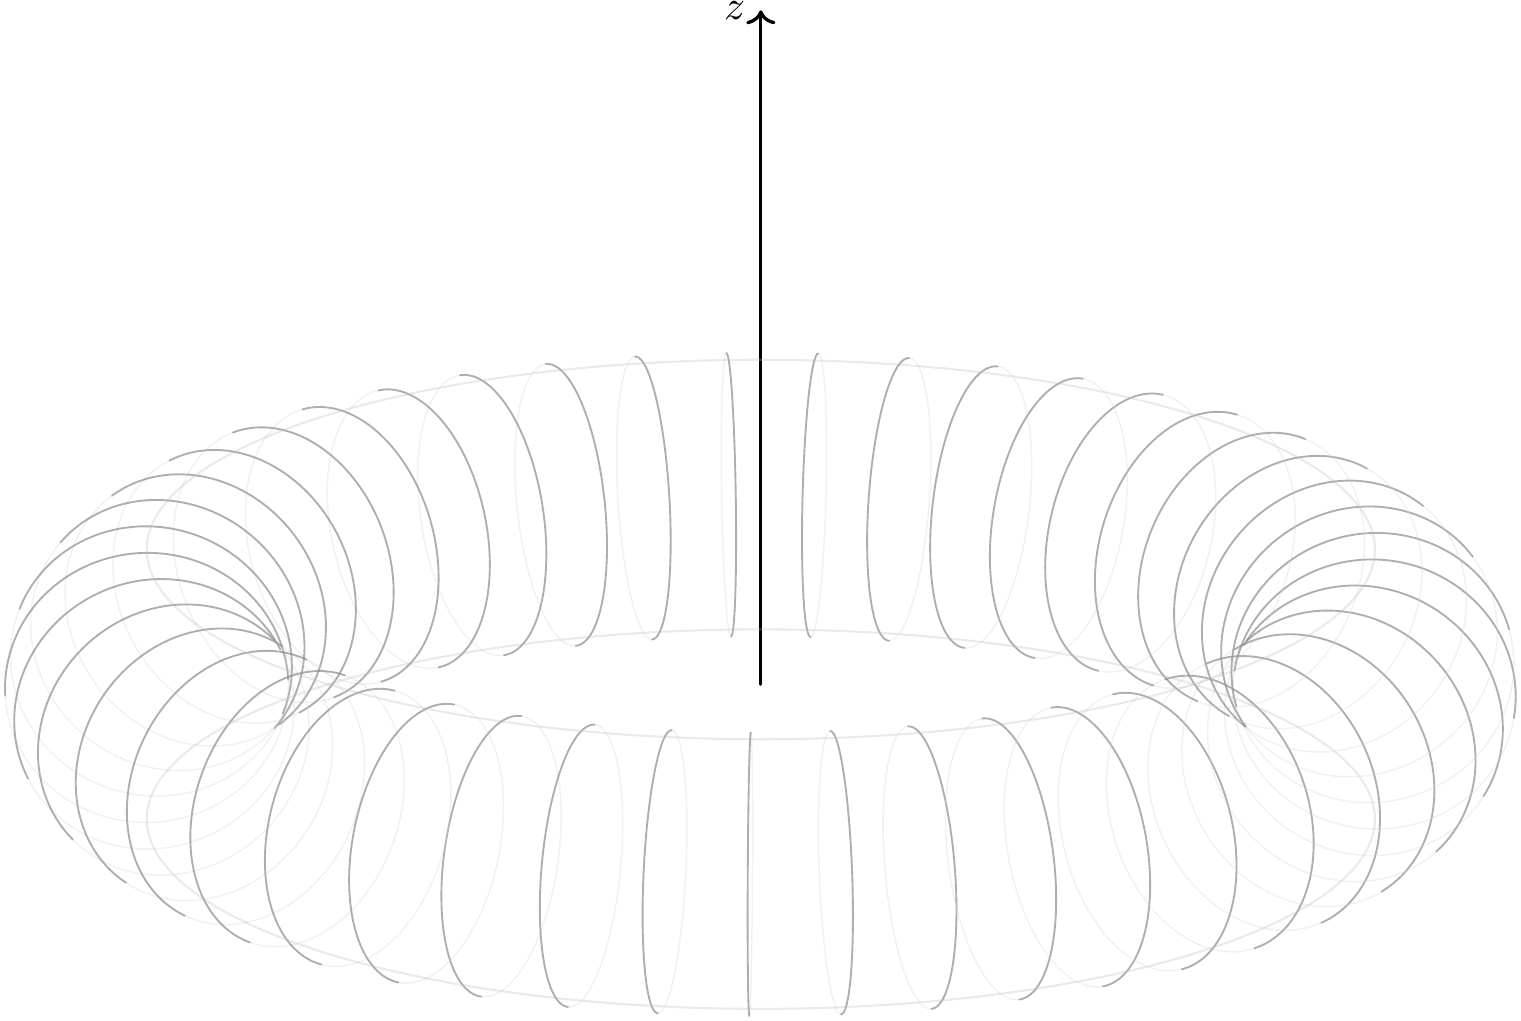
\includegraphics[width=\textwidth]{stf_multipole_expansion_fig/toroidal_electric_dipole_moment.png}
		\caption{环形电偶极矩}
		\label{环形偶极矩示意图-环形电偶极矩}
	\end{subfigure}
	\hfill
	\begin{subfigure}[b]{0.45\textwidth}
		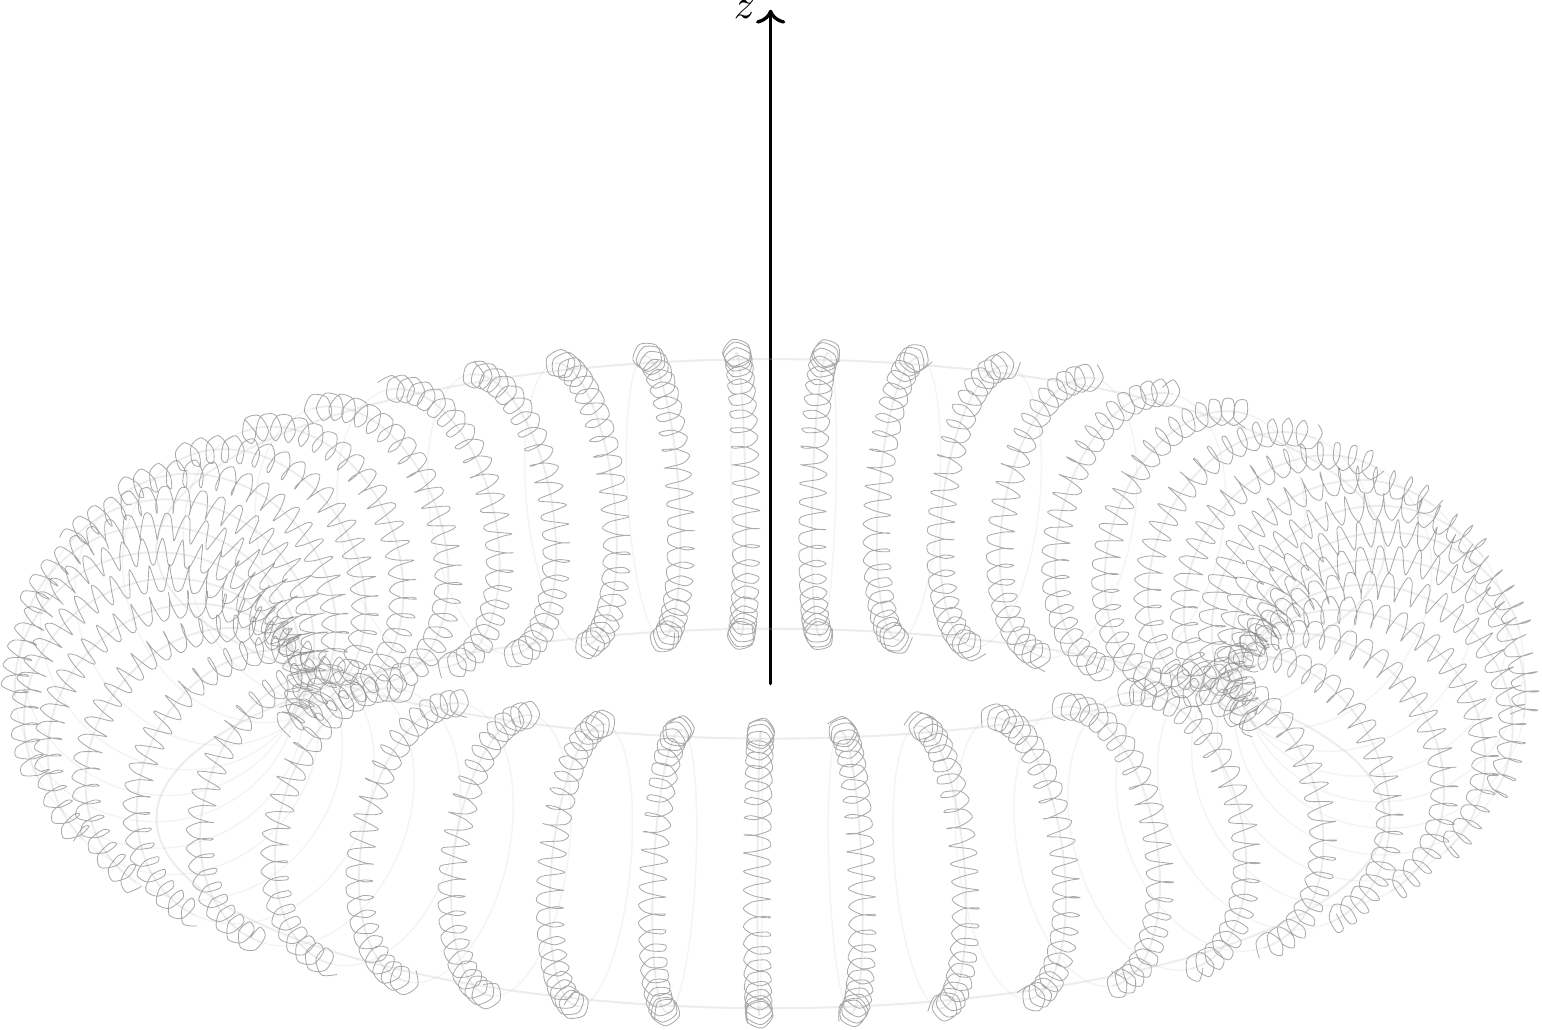
\includegraphics[width=\textwidth]{stf_multipole_expansion_fig/toroidal_magnetic_dipole_moment.png}
		\caption{环形磁偶极矩}
		\label{环形偶极矩示意图-环形磁偶极矩}
	\end{subfigure}
	\caption{环形偶极矩示意图}
	\label{环形偶极矩示意图}
\end{figure}